 \documentclass[handout,nooutcomes,noauthor,hints]{../ximera}

\graphicspath{  
{./}
{./whoAreYou/}
{./drawingWithTheTurtle/}
{./bisectionMethod/}
{./circles/}
{./anglesAndRightTriangles/}
{./lawOfSines/}
{./lawOfCosines/}
{./plotter/}
{./staircases/}
{./pitch/}
{./qualityControl/}
{./symmetry/}
{./nGonBlock/}
}


%% page layout
\usepackage[cm,headings]{fullpage}
\raggedright
\setlength\headheight{13.6pt}


%% fonts
\usepackage{euler}

\usepackage{FiraMono}
\renewcommand\familydefault{\ttdefault} 
\usepackage[defaultmathsizes]{mathastext}
\usepackage[htt]{hyphenat}

\usepackage[T1]{fontenc}
\usepackage[scaled=1]{FiraSans}

%\usepackage{wedn}
\usepackage{pbsi} %% Answer font


\usepackage{cancel} %% strike through in pitch/pitch.tex


%% \usepackage{ulem} %% 
%% \renewcommand{\ULthickness}{2pt}% changes underline thickness

\tikzset{>=stealth}

\usepackage{adjustbox}

\setcounter{titlenumber}{-1}

%% journal style
\makeatletter
\newcommand\journalstyle{%
  \def\activitystyle{activity-chapter}
  \def\maketitle{%
    \addtocounter{titlenumber}{1}%
                {\flushleft\small\sffamily\bfseries\@pretitle\par\vspace{-1.5em}}%
                {\flushleft\LARGE\sffamily\bfseries\thetitlenumber\hspace{1em}\@title \par }%
                {\vskip .6em\noindent\textit\theabstract\setcounter{question}{0}\setcounter{sectiontitlenumber}{0}}%
                    \par\vspace{2em}
                    \phantomsection\addcontentsline{toc}{section}{\thetitlenumber\hspace{1em}\textbf{\@title}}%
                     }}
\makeatother



%% thm like environments
\let\question\relax
\let\endquestion\relax

\newtheoremstyle{QuestionStyle}{\topsep}{\topsep}%%% space between body and thm
		{}                      %%% Thm body font
		{}                              %%% Indent amount (empty = no indent)
		{\bfseries}            %%% Thm head font
		{)}                              %%% Punctuation after thm head
		{ }                           %%% Space after thm head
		{\thmnumber{#2}\thmnote{ \bfseries(#3)}}%%% Thm head spec
\theoremstyle{QuestionStyle}
\newtheorem{question}{}



\let\freeResponse\relax
\let\endfreeResponse\relax

%% \newtheoremstyle{ResponseStyle}{\topsep}{\topsep}%%% space between body and thm
%% 		{\wedn\bfseries}                      %%% Thm body font
%% 		{}                              %%% Indent amount (empty = no indent)
%% 		{\wedn\bfseries}            %%% Thm head font
%% 		{}                              %%% Punctuation after thm head
%% 		{3ex}                           %%% Space after thm head
%% 		{\underline{\underline{\thmname{#1}}}}%%% Thm head spec
%% \theoremstyle{ResponseStyle}

\usepackage[tikz]{mdframed}
\mdfdefinestyle{ResponseStyle}{leftmargin=1cm,linecolor=black,roundcorner=5pt,
, font=\bsifamily,}%font=\wedn\bfseries\upshape,}


\ifhandout
\NewEnviron{freeResponse}{}
\else
%\newtheorem{freeResponse}{Response:}
\newenvironment{freeResponse}{\begin{mdframed}[style=ResponseStyle]}{\end{mdframed}}
\fi



%% attempting to automate outcomes.

%% \newwrite\outcomefile
%%   \immediate\openout\outcomefile=\jobname.oc
%% \renewcommand{\outcome}[1]{\edef\theoutcomes{\theoutcomes #1~}%
%% \immediate\write\outcomefile{\unexpanded{\outcome}{#1}}}

%% \newcommand{\outcomelist}{\begin{itemize}\theoutcomes\end{itemize}}

%% \NewEnviron{listOutcomes}{\small\sffamily
%% After answering the following questions, students should be able to:
%% \begin{itemize}
%% \BODY
%% \end{itemize}
%% }
\usepackage[tikz]{mdframed}
\mdfdefinestyle{OutcomeStyle}{leftmargin=2cm,rightmargin=2cm,linecolor=black,roundcorner=5pt,
, font=\small\sffamily,}%font=\wedn\bfseries\upshape,}
\newenvironment{listOutcomes}{\begin{mdframed}[style=OutcomeStyle]After answering the following questions, students should be able to:\begin{itemize}}{\end{itemize}\end{mdframed}}



%% my commands

\newcommand{\snap}{{\bfseries\itshape\textsf{Snap!}}}
\newcommand{\flavor}{\link[\snap]{https://snap.berkeley.edu/}}
\newcommand{\mooculus}{\textsf{\textbf{MOOC}\textnormal{\textsf{ULUS}}}}


\usepackage{tkz-euclide}
\tikzstyle geometryDiagrams=[rounded corners=.5pt,ultra thick,color=black]
\colorlet{penColor}{black} % Color of a curve in a plot



\ifhandout\newcommand{\mynewpage}{\newpage}\else\newcommand{\mynewpage}{}\fi


\title{Putting it all together}

\author{Claire Merriman}

\begin{document}
\begin{abstract}
Use the staircase data and program to answer questions.
\end{abstract}

\maketitle

\begin{listOutcomes}
 \item Use the staircase \snap\ program to answer questions using real world data,
 \item Modify the staircase \snap\ program for different regulations,
 \item Interpret solutions for the geometric issues of designing a staircase.
\item Reason through how to solve the geometric issues of designing a staircase.
\end{listOutcomes}

\begin{listObjectives}
 \item  Take a solution to a problem in a given context, and applying that same solution to another problem,
\item Learn and apply basic geometric formulas.
\end{listObjectives}

To start, get the following information from the \emph{Measuring Staircases} assignment:
\begin{itemize}
 \item Your group's staircase height \rule{2cm}{0.4pt}
 \item Your group's staircase length \rule{2cm}{0.4pt}
 \item The number of stairs in your group's staircase \rule{2cm}{0.4pt}
\end{itemize}

\begin{question}
Problem \ref{numberstairs} uses inches.  Problem \ref{cmstairs} uses centimeters. 

There are $2.54\ cm$ in $1\ in$. Use this fact to convert your group's data so that you can answer both questions. 
\end{question}

\mynewpage

\begin{question}\label{instructions}
Log into the \snap\ account you created the first week of class, then open the staircase.xml file.

To avoid issues with rounding, the first step of this problem is modifying the code to work with inches instead of feet.
 
Here are the instructions for editing the code:
\begin{enumerate}
 \item The code has the editable values: $5/6$ and $31/48$. Both of these values are in feet. Convert these to inches, keeping them as fractions. You can also get these values from the \emph{Staircases--Coding} assignment. Whole numbers can be written as a fraction where the denominator is $1$.
 \item Long press or right click on the block to bring up this menu: 
 
 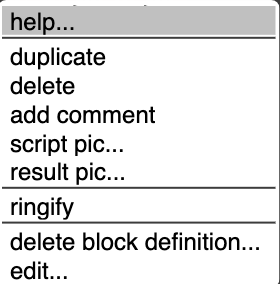
\includegraphics[height=1in]{snapmenu}
 
If you get a different menu, try pressing in a slightly different place. 
\item Select ``edit..." 
\item Change the values of $5/6$ and $31/48$ to inches.

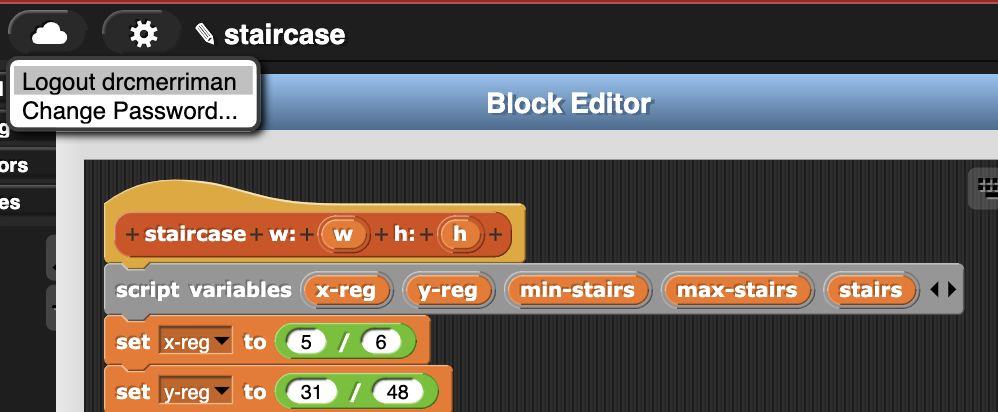
\includegraphics[width=.4\textwidth]{snapscreenshot}

\item With the block menu still open, select the cloud icon. Take a screenshot like the one above. \textbf{You need to include the edited \texttt{x-reg} and \texttt{y-reg} blocks, as well as your username. This should match your assignment from Week 1}.

\item Select ``OK".
\end{enumerate}

\textbf{Submit your screenshot as your answer to this question}. You will then use this code to answer the next question.
\end{question}

\mynewpage

\begin{question}\label{numberstairs}
Now that your code uses inches, input your staircase length for \texttt{w} and height for \texttt{h}.

Tab or left click on the block to see the results.  

You should get a spreadsheet with two or three rows and 3 columns.

Explain what the results mean in terms of number of stairs, riser height regulations, tread length regulations, staircase length, and staircase height. For example, here is a screenshot of the code from the \emph{Staircases--Coding} assignment 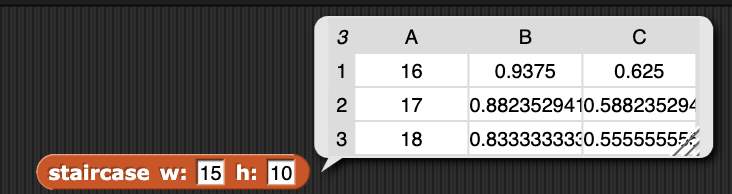
\includegraphics[height=1 in]{stairsfeet}

The output means that: If we want to build a staircase of length $15\ ft$ and height $10\ ft$ where the risers are at most $7\frac{3}{4}^{\prime\prime}$ tall and the treads are at least $10^{\prime\prime}$ long, we have must have at least $16\ stairs$ and at most $18\ stairs$. A staircase with $16\ stairs$ would have $0.9375\ ft$ long treads and $0.625\ ft$ high risers. A staircase with $17\ stairs$ would have $0.8824\ ft$ long treads and $0.5882\ ft$ high risers. 
A staircase with $18\ stairs$ would have $0.8333\ ft$ long treads and $0.5555\ ft$ high risers. 

Remember that the new input and output are in $inches$ not $feet$.

\end{question}
 
\mynewpage

\begin{question}
 The \emph{ArchDaily} article from the \emph{Measuring staircases} assignment does not give clear minimum and maximum values for riser heights and tread length. However, it does give a formula: \texttt{2 risers+ 1 tread= 63 to 65 cm}.

\begin{enumerate}
\item Use this formula to find a maximum riser height when the tread length is $25\ cm$. Show your calculations or otherwise explain how you found your answer.
\item Repeat the process from Problem \ref{instructions}, but change the $5/6$ to $25/1$ and the $31/48$ to the maximum height in centimeters. Submit a screenshot of your work.
\end{enumerate}
\end{question}

\begin{question}\label{cmstairs}
Now input your group's length and width values in centimeters. What differences are there in the output to this question that question \ref{numberstairs}? What causes those differences, in terms of in terms of number of stairs, riser height regulations, tread length regulations, staircase length, and staircase height. 
\end{question}
\end{document}